\documentclass{ximera}

\begin{document}
\textbf{For problems 1--3,} let $\vec{a} = \vector{-2,2}$ and $\vec{b}= \vector{4,2}$.

\begin{problem}
  Give a calculator-ready expression for the \textbf{angle} between $\vec{a}$
  and $\vec{b}$.


  \begin{prompt}
    \[
    \text{angle} = \answer{\arccos(-1/\sqrt{10})}
    \]
  \end{prompt}
  \vspace{1in}
  
\end{problem}


\begin{problem}
  \textbf{Sketch} and \textbf{label} $\vec{a}$, $\vec{b}$, and $\proj_{\vec{a}}(\vec{b})$.
  \begin{image}[3in]
    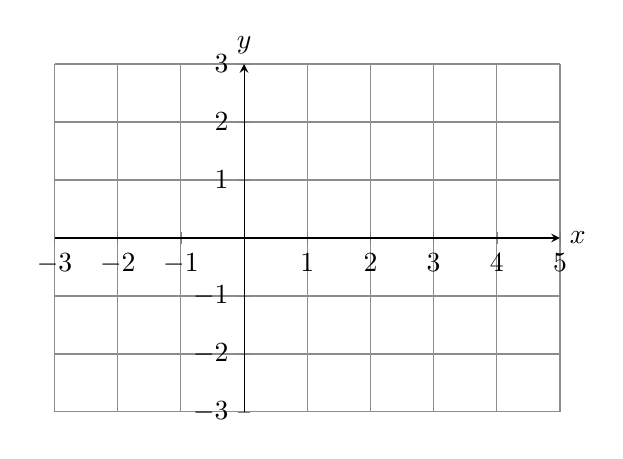
\begin{tikzpicture}
      \begin{axis}[
          xmin=-3,xmax=5,ymin=-3,ymax=3,
          clip=false,
          axis lines=center,
          width=8cm,
          height=6cm,
          xtick={-3,-2,...,5},
          ytick={-3,-2,...,3},
          xlabel=$x$, ylabel=$y$,
          grid=both,
          grid style={draw=gray!90},major grid style={draw=gray!90},
          minor tick num=0,
          every axis y label/.style={at=(current axis.above origin),anchor=south},
          every axis x label/.style={at=(current axis.right of origin),anchor=west},
        ]
        %\addplot[very thick,black,->] plot coordinates {(1,1) (4,2)};
        %\addplot[very thick,black,->] plot coordinates {(-1,0) (-3,3)};
        %\node[above] at (axis cs:2.5, 1.5) {$\vec{w}$};
        %\node[above] at (axis cs:-2, 1.5) {$\vec{v}$};
      \end{axis}
    \end{tikzpicture}
  \end{image}
  \begin{prompt}
    \begin{multipleChoice}
      \choice[correct]{I've done this.}
    \end{multipleChoice}
    \begin{feedback}
        \begin{image}[3in]
    \begin{tikzpicture}
      \begin{axis}[
          xmin=-3,xmax=5,ymin=-3,ymax=3,
          clip=false,
          axis lines=center,
          width=8cm,
          height=6cm,
          xtick={-3,-2,...,5},
          ytick={-3,-2,...,3},
          xlabel=$x$, ylabel=$y$,
          grid=both,
          grid style={draw=gray!90},major grid style={draw=gray!90},
          minor tick num=0,
          every axis y label/.style={at=(current axis.above origin),anchor=south},
          every axis x label/.style={at=(current axis.right of origin),anchor=west},
        ]
        \addplot[very thick,penColor,->] plot coordinates {(0,0) (-2,2)};
        \addplot[very thick,penColor2,->] plot coordinates {(0,0) (4,2)};
        \addplot[ultra thick,penColor3,->] plot coordinates {(0,0) (1,-1)};
        \addplot[black,dashed] plot coordinates {(1,-1) (4,2)};
        \node[below,penColor] at (axis cs:-1, 1) {$\vec{a}$};
        \node[above,penColor2] at (axis cs:2, 1) {$\vec{b}$};
        \node[below left,penColor3] at (axis cs:.5, -.5) {$\proj_{\vec{a}}(\vec{b})$};
      \end{axis}
    \end{tikzpicture}
  \end{image}
    \end{feedback}
  \end{prompt}
\end{problem}

\begin{problem}
  Find vectors $\vec{v}$ and $\vec{w}$ such that $\vec{v}$ is
  \textbf{parallel} to $\vec{a}$, $\vec{w}$ is \textbf{perpendicular}
  to $\vec{a}$, and $\vec{v}+\vec{w}=\vec{b}$. You may write the
  components of these vectors as calculator-ready expressions.
 
  \vfill
\end{problem}

\hrule

\begin{problem}
  \begin{selectAll}
    \pdfOnly{\begin{multicols}{2}}
    \choice{Let $\vec{f}:\R\to\R^3$. If $|\vec{f}(t)| = 2$ and $|\vec{f}'(t)| = 3$ \\ for all $t$, then $|\vec{f}(t) \dotp \vec{f}'(t)| = 6$.}
    \choice[correct]{Working in three-dimensional space, $\R^3$, \\ $y=x$ plots a plane.}
    \choice{Working in three-dimensional space, $\R^3$, \\ $(x-2)^2 +(z+1)^2 = 9$ plots a circle of radius $3$ \\ centered at $(2,0,-1)$.}
    \choice{The cross product of two unit vectors \\ is always a unit vector.}
    \choice[correct]{The plane $4x + 3y-z=0$ is perpendicular \\ to the line $x=4t$, $y=3t$, $z=-t$.}
    \columnbreak
    \choice[correct]{$\vector{2,-1}+\vector{\cos(t),\sin(t)}$ is parameterized by arc length.}
    \choice[correct]{If the distance between points $P$ and $Q$ is zero, \\ then $P=Q$.}
    \choice{If $\vec{q}'(t) = \vector{e^t,\sin(t),3t^2}$ and $\vec{q}(0) = \vector{4,1,2}$, then $\vec{q}(t) = \vector{e^t+4,-\cos(t)+1,t^3+2}$.}
    \choice{$\vector{2,1}+t\cdot \vector{\cos(t),\sin(t)}$ is parameterized by arc length.}
    \choice[correct]{$\proj_{\vec{w}}(\vec{w}) = \vec{w}$.}
    \pdfOnly{\end{multicols}}
    \end{selectAll}
\end{problem}


\end{document}
